%%%%%%%%%%%%%%%%%%%%%%%%%%%%%%%%%%%%%%%%%
% Beamer Presentation - LaTeX Template
% Version 2.0 (March 8, 2022)
% Original Template: https://www.LaTeXTemplates.com
% Author: Vel (vel@latextemplates.com)
% License: CC BY-NC-SA 4.0
%%%%%%%%%%%%%%%%%%%%%%%%%%%%%%%%%%%%%%%%%

%%%%%%%%%%%%%%%%%%%%%%%%%%%%%%%%%%%%%%%%%
% Este modelo de apresentação foi 
% criado a partir do modelo de Giovanni Spadaro.
% Disponível em: 
% https://github.com/Giovo17/presentation-template-unict-lm-data
%
% Adaptado por Lucas Amaral Taylor para criar uma versão especial 
% para os alunos de Matemática e Estatística da USP (IME-USP).
% Disponível em:
% https://github.com/lucasamtaylor01/IME-template
%%%%%%%%%%%%%%%%%%%%%%%%%%%%%%%%%%%%%%%%%

\documentclass[
	11pt, % Tamanho padrão da fonte
	% t, % Alinhar verticalmente ao topo
	%aspectratio=169, % Definir proporção 16:9
]{beamer}

% Caminho para imagens
\graphicspath{{img/}}

% Pacotes adicionais
\usepackage[alf]{abntex2cite} % Citações ABNT
\usepackage{booktabs} % Linhas de tabela aprimoradas
\usepackage{palatino} % Fonte Palatino
\usepackage[default]{opensans} % Fonte Open Sans
\usepackage{subcaption}
%----------------------------------------------------------------------------------------
%	PACOTES E CONFIGURAÇÕES PARA CÓDIGO
%----------------------------------------------------------------------------------------
% Pacotes necessários para formatação de código
\usepackage[utf8]{inputenc}
\usepackage{listings}
\usepackage{xcolor}

% Cores para syntax highlighting (VSCode Light Theme)
\definecolor{vscBackground}{RGB}{255,255,255}    % Fundo branco
\definecolor{vscKeyword}{RGB}{175,0,219}         % Roxo para palavras-chave
\definecolor{vscString}{RGB}{163,21,21}          % Vermelho para strings
\definecolor{vscComment}{RGB}{0,128,0}           % Verde para comentários
\definecolor{vscFunction}{RGB}{121,94,38}        % Marrom para funções
\definecolor{vscNumber}{RGB}{9,134,88}           % Verde escuro para números
\definecolor{vscOperator}{RGB}{175,0,219}        % Roxo para operadores
\definecolor{vscText}{RGB}{0,0,0}                % Texto preto
\definecolor{vscLineNr}{RGB}{128,128,128}        % Cinza para números de linha

% Configuração geral do listings para UTF-8
\lstset{
    inputencoding=utf8,
    extendedchars=true,
    literate=%
        {á}{{\'a}}1 {é}{{\'e}}1 {í}{{\'i}}1 {ó}{{\'o}}1 {ú}{{\'u}}1
        {Á}{{\'A}}1 {É}{{\'E}}1 {Í}{{\'I}}1 {Ó}{{\'O}}1 {Ú}{{\'U}}1
        {à}{{\`a}}1 {è}{{\`e}}1 {ì}{{\`i}}1 {ò}{{\`o}}1 {ù}{{\`u}}1
        {À}{{\`A}}1 {È}{{\'E}}1 {Ì}{{\`I}}1 {Ò}{{\`O}}1 {Ù}{{\`U}}1
        {ã}{{\~a}}1 {ẽ}{{\~e}}1 {ĩ}{{\~i}}1 {õ}{{\~o}}1 {ũ}{{\~u}}1
        {Ã}{{\~A}}1 {Ẽ}{{\~E}}1 {Ĩ}{{\~I}}1 {Õ}{{\~O}}1 {Ũ}{{\~U}}1
        {â}{{\^a}}1 {ê}{{\^e}}1 {î}{{\^i}}1 {ô}{{\^o}}1 {û}{{\^u}}1
        {Â}{{\^A}}1 {Ê}{{\^E}}1 {Î}{{\^I}}1 {Ô}{{\^O}}1 {Û}{{\^U}}1
        {ç}{{\c c}}1 {Ç}{{\c C}}1
        {º}{{\textordmasculine}}1
        {ª}{{\textordfeminine}}1
}

% Configurações base comum para todas as linguagens
\lstdefinestyle{baseStyle}{
    backgroundcolor=\color{vscBackground},
    basicstyle=\ttfamily\small\color{vscText},
    breakatwhitespace=false,
    breaklines=true,
    captionpos=b,
    keepspaces=true,
    numbers=left,
    numbersep=5pt,
    showspaces=false,
    showstringspaces=false,
    showtabs=false,
    tabsize=4,
    frame=single,
    framerule=0.8pt,
    rulecolor=\color{gray!20},
    numberstyle=\tiny\color{vscLineNr},
    keywordstyle=\color{vscKeyword},
    commentstyle=\color{vscComment}\itshape,
    stringstyle=\color{vscString},
    emphstyle=\color{vscFunction},
    columns=flexible,
    basewidth={0.5em,0.45em},
    inputencoding=utf8,
    extendedchars=true
}

%----------------------------------------------------------------------------------------
% Python
%----------------------------------------------------------------------------------------
\lstdefinestyle{pythonStyle}{
    style=baseStyle,
    language=Python,
    morekeywords={self,None,True,False,import,from,as,def,class,return,yield,
                  for,while,if,else,elif,try,except,finally,with,lambda,
                  async,await,break,continue,global,nonlocal,pass,raise},
    morekeywords=[2]{print,len,range,type,int,str,float,list,dict,set,
                     tuple,max,min,sum,sorted,enumerate,zip,map,filter,
                     any,all,abs,round,pow,divmod},
    keywordstyle=[2]\color{vscFunction},
    sensitive=true
}

\lstnewenvironment{python}[1][]{\lstset{style=pythonStyle, #1}}{}
\newcommand{\pyinline}[1]{\lstinline[style=pythonStyle]!#1!}
\newcommand{\inputpython}[2][]{\lstinputlisting[style=pythonStyle,#1]{#2}}

%----------------------------------------------------------------------------------------
% C Language
%----------------------------------------------------------------------------------------
\lstdefinestyle{cStyle}{
    style=baseStyle,
    language=C,
    morekeywords={include,define,void,int,char,float,double,long,unsigned,
                  struct,union,enum,typedef,const,static,extern,register,
                  auto,volatile,sizeof,return,if,else,for,while,do,switch,
                  case,break,continue,default,goto},
    morekeywords=[2]{printf,scanf,malloc,free,calloc,realloc,fopen,fclose,
                     fprintf,fscanf,strcpy,strlen,strcat},
    keywordstyle=[2]\color{vscFunction},
    sensitive=true
}

\lstnewenvironment{clang}[1][]{\lstset{style=cStyle, #1}}{}
\newcommand{\clinline}[1]{\lstinline[style=cStyle]!#1!}
\newcommand{\inputclang}[2][]{\lstinputlisting[style=cStyle,#1]{#2}}

%----------------------------------------------------------------------------------------
% C++
%----------------------------------------------------------------------------------------
\lstdefinestyle{cppStyle}{
    style=baseStyle,
    language=C++,
    morekeywords={class,private,protected,public,template,typename,namespace,
                  using,new,delete,this,friend,virtual,override,final,explicit,
                  mutable,constexpr,nullptr,noexcept,static_cast,dynamic_cast,
                  const_cast},
    morekeywords=[2]{cout,cin,endl,vector,string,map,set,queue,stack,pair,
                     begin,end,push_back,pop_back,emplace_back,size,empty},
    keywordstyle=[2]\color{vscFunction},
    sensitive=true
}

\lstnewenvironment{cpp}[1][]{\lstset{style=cppStyle, #1}}{}
\newcommand{\cppinline}[1]{\lstinline[style=cppStyle]!#1!}
\newcommand{\inputcpp}[2][]{\lstinputlisting[style=cppStyle,#1]{#2}}

%----------------------------------------------------------------------------------------
% R Language
%----------------------------------------------------------------------------------------
\lstdefinestyle{rStyle}{
    style=baseStyle,
    language=R,
    morekeywords={if,else,repeat,while,function,for,in,next,break,TRUE,FALSE,
                  NULL,Inf,NaN,NA,NA_integer_,NA_real_,NA_complex_,NA_character_},
    morekeywords=[2]{library,require,attach,detach,source,setwd,options,
                     data.frame,read.csv,write.csv,list,matrix,array},
    keywordstyle=[2]\color{vscFunction},
    sensitive=true
}

\lstnewenvironment{rlang}[1][]{\lstset{style=rStyle, #1}}{}
\newcommand{\rlinline}[1]{\lstinline[style=rStyle]!#1!}
\newcommand{\inputrlang}[2][]{\lstinputlisting[style=rStyle,#1]{#2}}

%----------------------------------------------------------------------------------------
% Java
%----------------------------------------------------------------------------------------
\lstdefinestyle{javaStyle}{
    style=baseStyle,
    language=Java,
    morekeywords={abstract,assert,boolean,break,byte,case,catch,char,class,
                  const,continue,default,do,double,else,enum,extends,final,
                  finally,float,for,if,implements,import,instanceof,int,
                  interface,long,native,new,package,private,protected,public,
                  return,short,static,strictfp,super,switch,synchronized,this,
                  throw,throws,transient,try,void,volatile,while},
    morekeywords=[2]{String,System,out,println,printStackTrace,ArrayList,
                     HashMap,Arrays,List,Map,Set,Exception,RuntimeException},
    keywordstyle=[2]\color{vscFunction},
    sensitive=true
}

\lstnewenvironment{java}[1][]{\lstset{style=javaStyle, #1}}{}
\newcommand{\javainline}[1]{\lstinline[style=javaStyle]!#1!}
\newcommand{\inputjava}[2][]{\lstinputlisting[style=javaStyle,#1]{#2}} % Código

%----------------------------------------------------------------------------------------
%	SELEÇÃO DE LAYOUT E CORES
%----------------------------------------------------------------------------------------

\usetheme{Boadilla} % Tema de layout

% Definição de cores personalizadas
\definecolor{primaryColor}{RGB}{20,45,105} % Cor primária
\definecolor{secondaryColor}{RGB}{0,100,160} % Cor secundária

% Aplicação das cores no tema
\setbeamercolor{structure}{fg=primaryColor}
\setbeamercolor{palette primary}{bg=primaryColor, fg=white}
\setbeamercolor{palette secondary}{bg=secondaryColor, fg=white}
\setbeamercolor{title}{bg=primaryColor, fg=white} % Cor do título principal

% Cores no cabeçalho
\setbeamercolor{headline}{bg=secondaryColor, fg=white}
\setbeamercolor{section in head/foot}{bg=primaryColor, fg=white}
\setbeamercolor{subsection in head/foot}{bg=secondaryColor, fg=white}

% Configurações de cores para o rodapé
\setbeamercolor{author in head/foot}{bg=primaryColor, fg=white} % Nome
\setbeamercolor{title in head/foot}{bg=secondaryColor, fg=white} % Título
\setbeamercolor{date in head/foot}{bg=primaryColor, fg=white} % Ano
\setbeamercolor{page number in head/foot}{bg=primaryColor, fg=white} % Página

% Temas internos e externos
\useinnertheme{circles} % Tema interno
\useoutertheme{miniframes} % Tema externo
\setbeamertemplate{navigation symbols}{} % Remove símbolos de navegação

%------------------
%	INFORMAÇÕES DA APRESENTAÇÃO
%------------------

\title[Répondération ]{TRAITEMENT DE NON REPONSE TOTALE}
\author[Traitement de la non-réponse totale]{Presenté par : \\ Crépin  MEDEHOUIN  \vspace{0.8cm}  } 

\institute[]{Formateur : Dr. KOUAME Darès } 
\date[2024 - 2025]{} 

%------------------

\begin{document}

%------------------
%	SLIDE DE TÍTULO
%------------------

\begin{frame}
	\begin{figure}
		
\includegraphics[width=0.45\linewidth]{img/logo_ensea.png}
	\end{figure}
	\titlepage % Exibe o slide de título
\end{frame}

%------------------
%	SLIDE DE ÍNDICE
%------------------

\begin{frame}
	\frametitle{PLAN} % Título do slide
	\tableofcontents % Exibe o índice
\end{frame}

%------------------
%	SEÇÕES DO CORPO DA APRESENTAÇÃO
%------------------

\section{Introduction} % Seções são adicionadas para organizar sua apresentação em blocos discretos, todas as seções e subseções são automaticamente exibidas no índice como uma visão geral da apresentação, mas NÃO são exibidas como slides separados.

%------------------------------------------------
\begin{frame}{}
	
	\huge \begin{center}
		INTRODUCTION
	\end{center}
	
\end{frame}

\begin{frame}
	\frametitle{Introduction}
  


On dit qu'il y a non-réponse vis-à-vis de la variable Y pour l'individu échantillonné i dès lors que l'on ne dispose pas de la valeur $Y_i$ relative à cet individu. \\ \vspace{0.5cm}
 On distingue deux types de non réponse :
  \begin{enumerate}
  	\item les non réponses totales 
  	\item les non réponses partielles
  \end{enumerate}
 
\end{frame}


\begin{frame}
	\frametitle{Introduction}
	
La \textbf{non-réponse totale} est habituellement traitée par une méthode de \textbf{repondération}: \vspace{0.5cm}
	
\begin{enumerate}
\item	on supprime du fichier les non-répondants totaux,
\item	on augmente les poids des répondants pour compenser de la non-réponse totale.
\end{enumerate} 

\vspace{0.5cm}

La non-réponse partielle est habituellement traitée par imputation $\Rightarrow$
une valeur manquante est remplacée par une valeur plausible.


\end{frame}

\begin{frame}
	\frametitle{Introduction}

\textbf{L’objectif prioritaire} est de \textbf{réduire} autant que possible \textbf{le biais de
non-réponse} : cela passe par une recherche des facteurs explicatifs de la non-réponse

\end{frame}


%------------------------------------------------

%------------------------------------------------

\begin{frame}
	\frametitle{Non réponses totales }
	
On a une non réponse totale lorsque l’on n’a aucune donnée sur l’unité d’observation. \\ \vspace{0.5cm}

Autrement dit, on a aucune réponse aux questions posées. Cela ne signifie pas que l'on ne dispose aucune information sur le non-répondant : \\  \vspace{0.5cm}

En général, on dispose tout de même de renseignements présents dans la base de sondage, ou collectés sur le terrain (Par exemple des renseignements obtenus auprès de tierces personnes)


    %\begin{itemize}
     %   \item Lorem ipsum dolor sit amet.
      %  \item Lorem ipsum dolor sit amet.
    %\end{itemize}
	
\end{frame}



\begin{frame}
	\frametitle{Non réponses totales }
On va traiter ce problème par \textbf{repondération} : on fait porter aux répondants le poids des non-répondants. Cette repondération se justifie sous une modélisation du mécanisme de non-réponse.\\ \vspace{0.5cm}
Cette modélisation permet d’estimer les probabilités de réponse à
l’enquête, pour obtenir les poids corrigés de la non-réponse totale.
\end{frame}

\begin{frame}
	\frametitle{Quelques facteurs de non-réponse totale (Haziza, 2011)}
	
\begin{itemize}
	\item Mauvaise qualité de la base de sondage;
	\item Impossibilité de joindre l’individu;
	\item Type d’enquête (obligatoire ou volontaire);
	\item Fardeau de réponse;
	\item Méthode de collecte (interview, téléphone, courrier, ...);
	\item Durée de collecte;
	\item Suivi (et relance) des non-répondants;
    \item Formation des enquêteurs.
\end{itemize}

\end{frame}



\begin{frame}
	\frametitle{Hors champs}
	
Un point important : la distinction entre individus hors-champ et individus non-répondants \\ \vspace{0.4cm}


On parle de hors champs quand une valeur manquante est dû au fait que l’enquêté n’est pas concerné par la question : \\ \vspace{0.4cm}

\begin{enumerate}
	\item S'il concerne toute les variables, elle est total (HCT) 
	\item Ou partiel s’il concerne quelques variables (HCP) 
\end{enumerate} 

 \vspace{0.3cm}
La non réponses modifie les poids de sondage alors que le hors champs ne les modifie pas.
\end{frame}









\section{Principe de repondération} % Seções são adicionadas para organizar sua apresentação em blocos discretos, todas as seções e subseções são automaticamente exibidas no índice como uma visão geral da apresentação, mas NÃO são exibidas como slides separados.

%------------------------------------------------
\begin{frame}{}
	
	\huge \begin{center}
		PRINCIPE
	\end{center}
	
\end{frame}


\begin{frame}
	\frametitle{Les étapes du traitement de la non-réponse totale }
	

\vspace{0.5cm}
\begin{enumerate}
\item Identification des non-répondants,
\item Modélisation du mécanisme de non-réponse (recherche des facteurs explicatifs),
\item Estimation des probabilités de réponse,
\item Calcul des poids corrigés de la non-réponse totale.
\end{enumerate}

\end{frame}

\begin{frame}
	\frametitle{Modélisation du mécanisme de non-réponse}
	
On note $r_k$ la variable indicatrice de réponse pour l’individu k, valant
1 si l’individu a répondu à l’enquête et 0 sinon. \\ 

\[
r_k =
\begin{cases} 
	1 & \text{si l’individu $k$ a répondu}, \\
	0 & \text{sinon}.
\end{cases}
\]
\vspace{0.5cm}


On note $p_{k \mid S} \equiv p_k$ la probabilité de réponse pour l’unité $k$ : 
\[
p_k = \Pr(k \in S_r \mid S) = \Pr(r_k = 1 \mid S).
\]

\end{frame}


\begin{frame}
	\frametitle{Modélisation du mécanisme de non-réponse}

Si on veut estimer le total T d'une variable dans l'échantillon total, T est estimé sans biais par l’estimateur de \textbf{Horvitz-Thompson} : $$ \hat{T} = \sum_{k \in S} w_k y_k = \sum_{k \in S} \frac{y_k}{\pi_k}  $$

avec $w_k = \frac{1}{\pi_k}$ le poids de sondage de l’unité $k$ \\  \vspace{0.3cm}

En présence de non réponse totale, on obtient un estimateur sans biais du total T : $$\hat{T}_r =  \sum_{k \in S_r} \frac{y_k}{\pi_k \times p_k}$$
\end{frame}

\begin{frame}{}
	\begin{figure}[h]
		\centering
		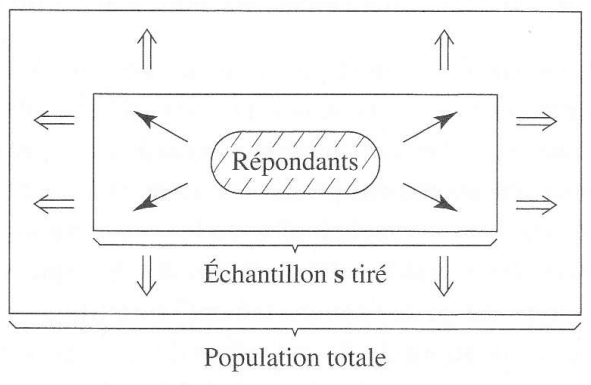
\includegraphics[width=0.9\textwidth]{img/s.png}
		%	\caption{Legenda da imagem}
		%	\label{fig:label_da_imagem}
	\end{figure}
\end{frame}

\begin{frame}
	\frametitle{Hypothèses}



On fait l’hypothèse que :
\begin{itemize}
	\item toutes les probabilités de réponse vérifient $0 < p_k \leq 1$ : pas de non-répondants irréductibles,
	\item les individus répondent indépendamment les uns des autres : 
	\[
	\Pr(k, l \in S_r \mid S) \equiv p_{kl} = p_k p_l.
	\]
\end{itemize}
Cette dernière hypothèse peut être affaiblie (Haziza et Rao, 2003 ; Skinner et D’Arrigo, 2011).


\end{frame}



\begin{frame}
	\frametitle{Types de mécanisme}

On distingue schématiquement trois types de mécanisme de non-réponse :  \\ \vspace{0.5cm}
\begin{enumerate}
	\item uniforme (ou MCAR),
	\item ignorable (ou MAR),
	\item non-ignorable (ou NMAR).
\end{enumerate}

\end{frame}


 
\section{Différentes méthodes} % Seções são adicionadas para organizar sua apresentação em blocos discretos, todas as seções e subseções são automaticamente exibidas no índice como uma visão geral da apresentação, mas NÃO são exibidas como slides separados.

\begin{frame}{}
	
	\huge \begin{center}
		 Méthode de repondération uniforme
	\end{center}
	
\end{frame}


\begin{frame}{Mecanisme uniforme (ou MCAR)}
	
Le mécanisme est dit uniforme (ou Missing Completely At Random)
quand $p_k = p$, i.e. quand tous les individus ont la même probabilité
de réponse. \\ \vspace{0.5cm} 

C’est une hypothèse généralement peu réaliste. \\ \vspace{0.5cm}
\textbf{Exemple} : non-réponse provenant de la perte de questionnaires.
	
\end{frame}


\begin{frame}{Exemple}
	
	Prenons l'exemple d'une population de \textbf{10 personnes}, dans laquelle on tire \textbf{5 individus}
	par sondage aléatoire simple.  \\ \vspace{0.2cm}
	
	Supposons (cas d'école) que $y_k$ soit égal à 1 pour chacun des 10 individus, et que, \textbf{parmi les 5} personnes tirées, seulement \textbf{2 acceptent} de répondre.
	On a: \\ \vspace{0.2cm}
	
	$ N=10, \hspace{3mm} n =5 \hspace{3mm} $ et $ \hspace{3mm} \pi_k = f = \frac{n}{N} = \frac{1}{2} \hspace{3mm} $  pour  tout  k\\ \vspace{0.2cm}
	
	Le vrai total est T = 10. Si on ne corrige pas des non-réponses, on utilise naivement : 
	$$\hat{T} =  \sum_{k \in S_r} \frac{y_k}{\pi_k} = \frac{1}{\frac{1}{2}} + \frac{1}{\frac{1}{2}} = 4$$
	
\end{frame}



\begin{frame}{Exemple}
	
	Puisqu'on ne dispose des valeurs $y_k$ que pour deux individus. T est manifestement un
	mauvais estimateur de T, fortement biaisé. \\ \vspace{0.3cm}
	
	Pour limiter ce biais, on peut cependant raisonner ainsi : \\ \vspace{0.3cm}
	
	sur les cinq personnes tirées, puisque deux répondent, on peut penser que chacune a une probabilité $r_k = \frac{2}{5} $ de répondre. \\ 
	
	$$\hat{T}_r =  \sum_{k \in S_r} \frac{y_k}{\pi_k \times p_k} =  \frac{1}{\frac{1}{2} \times \frac{2}{5}} + \frac{1}{\frac{1}{2}  \times \frac{2}{5}} = 10 $$
	
	
L'idée qui vient d'être	appliquée consiste à estimer la probatrilité de réponse supposée commune par un taux de réponse empirique. 
	
\end{frame}


\begin{frame}{Mecanisme uniforme (ou MCAR)}

La méthode de repondération uniforme est facile à mettre en œuvre et il n’y a pas de calcul complexe pour la probabilité de réponse et le fait
d’attribuer la même probabilité de réponse à chaque individu garantit un traitement équitable pour toutes les observations.\\ \vspace{0.5cm}

Cependant, cette
méthode ne tient pas en compte l’hétérogénéité des données


\end{frame}
%------------------------------------------------



%------------------------------------------------


\begin{frame}{}
	
	\huge \begin{center}
		Mécanisme de réponse homogène
	\end{center}
	
\end{frame}


\begin{frame}{Mécanisme de non-réponse ignorable (MAR)}
	
On parle de mécanisme de non-réponse ignorable (ou Missing At Random) quand les probabilités de réponse peuvent être expliquées à l’aide de l’information auxiliaire disponible : 
\[
\Pr(r_k = 1 \mid y_k, z_k) = \Pr(r_k = 1 \mid z_k),
\]
avec 
\begin{itemize}
	\item $y_k$ la variable d’intérêt,
	\item $z_k$ le vecteur des valeurs prises par un vecteur $\mathbf{z}$ de variables auxiliaires pour l’individu $k$ de $S$.
\end{itemize}

\textbf{Exemple :} enquête sur le revenu + non-réponse expliquée par le sexe des individus.

\end{frame}

\begin{frame}{Mécanisme de non-réponse ignorable (MAR)}

	
	Cette méthode consiste à repartir les unités de la population en
	sous-groupes disjoints appelés groupes de réponses homogènes. A
	l’intérieur de chaque groupe, les individus ont des comportements de
	réponse indépendants et une probabilité de réponse commune et non nulle.
	La probabilité de réponse est égale au rapport des unités répondants dans
	un groupe par le nombre d’unités dans le groupe.
	
	
\end{frame}

\begin{frame}{}
	\begin{figure}[h]
		\centering
		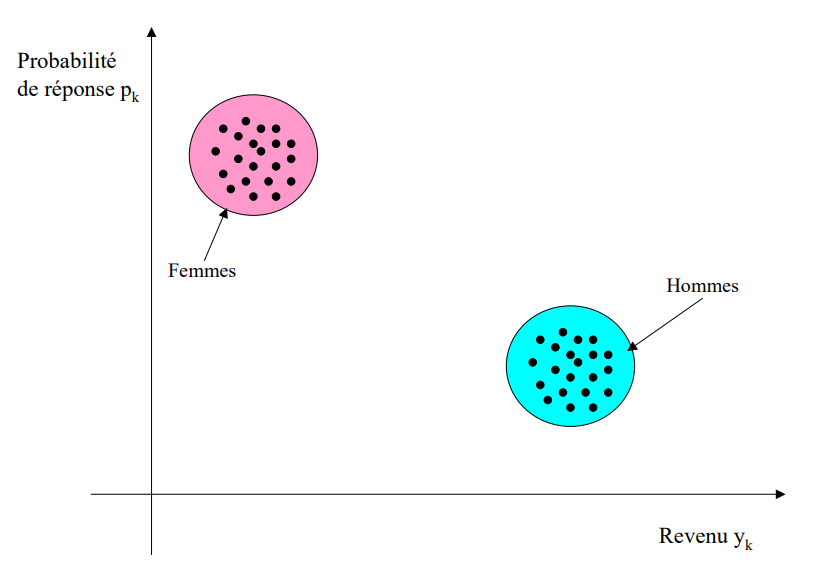
\includegraphics[width=0.9\textwidth]{img/sex.png}
		%	\caption{Legenda da imagem}
		%	\label{fig:label_da_imagem}
	\end{figure}
\end{frame}

\begin{frame}{Exemple}
	Dans une enquête sur le revenu, avec un échantillon initial de 10 000 personnes et un échantillon répondant de taille 8 000, il serait grossier d'estimer $r_k$ par 80\% pour chaque individu. \\ \vspace{0.3cm}
	
	Une solution plus satisfaisante consisterait à considérer les catégories socioprofessionnelles (CSP) si on en dispose pour chaque individu tiré, répondant ou non (ou, mieux, les croisements CSP - âge si l'information existe), et à estimer un taux de réponse
	par catégorie. \\ \vspace{0.3cm}
	
	En effet, il est très probable que les taux de réponse différeront fortement
	selon la catégorie, et on pouffa ainsi obtenir des estimations des $r_k$ plus proches dela réalité. \\ 
	
	
\end{frame}

\begin{frame}{Exemple}
	Par exemple, supposons que l'on obtienne :
	
	\begin{figure}[h]
		\centering
		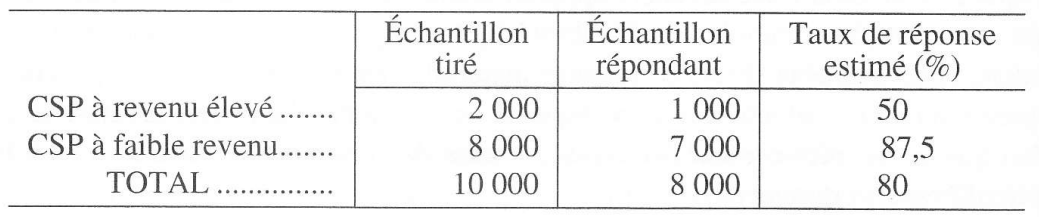
\includegraphics[width=1\textwidth]{img/e.png}
		%	\caption{Legenda da imagem}
		%	\label{fig:label_da_imagem}
	\end{figure}
	
	Ainsi, si $S_{r_1}$ désigne l'échantillon de répondants parmi les CSP à fort revenu (respectivement $S_{r_2}$, parmi les CSP à faible revenu), on utilisera : 
	$$ \hat{T}_r = \sum_{k \in S_{r_1}} \frac{y_k}{\pi_k \times 0.5} + \sum_{k \in S_{r_2}} \frac{y_k}{\pi_k \times 0.875}$$
	
\end{frame}


\begin{frame}{}
	
	\huge \begin{center}
		Le mécanisme de non-réponse ignorable (NMAR)
	\end{center}
	
\end{frame}



\begin{frame}{Mécanisme de non-réponse non ignorable (NMAR)}
Un mécanisme de non-réponse qui n’est pas ignorable est dit non-ignorable (ou Non Missing At Random). \vspace{0.3cm}

\textbf{Cela signifie que la non-réponse dépend de la variable d’intérêt, même une fois que l’on a pris en compte les variables auxiliaires}. \\ \vspace{0.5cm}

Il est très difficile de corriger de la non-réponse non ignorable, ou même de la détecter.\\ \vspace{0.5cm}

\textbf{Exemple :} enquête sur le revenu + non-réponse expliquée par le croisement sexe $\times$ revenu.

\end{frame}



\begin{frame}{Mécanisme de non-réponse ignorable (NMAR)}
	
En pratique, les probabilités de réponse $p_k$ sont inconnues et doivent être estimées. On postule alors un modèle de réponse de la forme 
\[
p_k = f(z_k, \beta_0),
\]
avec 
\begin{itemize}
	\item $z_k$ un vecteur de variables auxiliaires connu sur $S$,
	\item $f(\cdot, \cdot)$ une fonction connue,
	\item $\beta_0$ un paramètre inconnu.
\end{itemize}


\end{frame}

\begin{frame}{Mécanisme de non-réponse ignorable (NMAR)}
	
La liaison en question peut prendre les formes les plus diverses. Une des plus "célèbres" consiste à écrire :\\ 

$$r_k \simeq \frac{a.e^{bX_k}}{1+ a.e^{bX_k}} \Rightarrow Log \frac{r_k}{1+r_k} \simeq Log a + bX_k $$



On parle alors de modèle \textbf{LOGIT} et on sait mettre en œuvre
des procédures pour estimer les paramètres a et b selon certains critères optimaux

\end{frame}

\begin{frame}{Mécanisme de non-réponse ignorable (MAR)}
	
On peut aussi trouver d'autres fonctions de X, qui ont bonne allure et qui
sont toujours comprises entre 0 et 1. Par exemple, on peut s'appuyer sur la fonction de
répartition $\phi(x)$ d'une loi normale centrée réduite, soit


\[ \phi(x) = 
\int_{-\infty}^{x} \frac{1}{\sqrt{2\pi}} e^{-\frac{t^2}{2}} \, dt
\]


et ajuster le modèle $r_k \simeq \phi(a	+ bX_k)$
On parle cette fois de modèle \textbf{PROBIT}, et on sait
également estimer a et b par des techniques appropriées.

\end{frame}

\begin{frame}{}
	\begin{figure}[h]
		\centering
		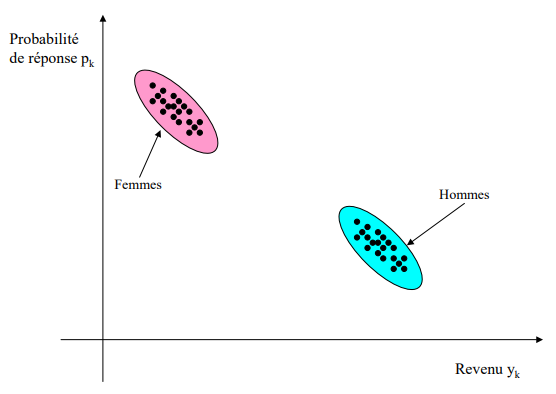
\includegraphics[width=0.9\textwidth]{img/re.png}
		%	\caption{Legenda da imagem}
		%	\label{fig:label_da_imagem}
	\end{figure}
\end{frame}

 
\section{Un cas pratique} % Seções são adicionadas para organizar sua apresentação em blocos discretos, todas as seções e subseções são automaticamente exibidas no índice como uma visão geral da apresentação, mas NÃO são exibidas como slides separados.

\begin{frame}{}
	
	\huge \begin{center}
		CAS PRATIQUE
	\end{center}
	

	
\end{frame}


 
\section{Conclusion} % Seções são adicionadas para organizar sua apresentação em blocos discretos, todas as seções e subseções são automaticamente exibidas no índice como uma visão geral da apresentação, mas NÃO são exibidas como slides separados.

\begin{frame}{}
	
	\huge \begin{center}
		Conclusion
	\end{center}
	
\end{frame}

\begin{frame}{Conclusion}
  
  En conclusion, les méthodes de repondération face aux non-réponses sont cruciales pour garantir la fiabilité des résultats d'enquête. La repondération uniforme, le mécanisme de réponse homogène, et l'estimation des probabilités de réponse permettent de corriger les biais liés aux non-réponses.\\ \vspace{0.4cm}
  
   Chacune présente des avantages et des limites selon le contexte. Leur choix doit être adapté aux spécificités de l’enquête et de la population cible. \\ \vspace{0.4cm}
  
  Une approche bien choisie améliore la représentativité des données et la qualité des analyses.
\end{frame}



\begin{frame}{Références}
	\begin{enumerate}
\item Ardilly, Pascal. 2006. Les Techniques de Sondage / Pascal Ardilly,... Éditions Technip. https://bibliotheque.univ-catholille.fr/Default/doc/SYRACUSE/340736/les-techniques-de-sondage-pascal-ardilly.\\ \vspace{0.5cm}
\item Chauvet, Guillaume. n.d. “Données Manquantes dans les Enquêtes.”
	\end{enumerate}


\end{frame} 

%------------------
%	SLIDE DE ENCERRAMENTO
%------------------

\begin{frame}
	\begin{center}
		{\Huge MERCI POUR VOTRE \\ }
		{\Huge \vspace{0.5cm}}
		{\Huge ATTENTION}
	\end{center}
\end{frame}

%------------------

\end{document}
